%%%%%%%%%%%%%%%%%%%%%%%%%%%%%%%%%%%%%%%%%
% Stylish Article
% LaTeX Template
% Version 2.1 (1/10/15)
%
% This template has been downloaded from:
% http://www.LaTeXTemplates.com
%
% Original author:
% Mathias Legrand (legrand.mathias@gmail.com) 
% With extensive modifications by:
% Vel (vel@latextemplates.com)
%
% Authors:
% Mauricio Hoyos Ardila mhoyosa2@eafit.edu.co
% Jonathan Zapata Castaño jzapat80@eafit.edu.co
%
% License:
% CC BY-NC-SA 3.0 (http://creativecommons.org/licenses/by-nc-sa/3.0/)
%
%%%%%%%%%%%%%%%%%%%%%%%%%%%%%%%%%%%%%%%%%

%----------------------------------------------------------------------------------------
%	PACKAGES AND OTHER DOCUMENT CONFIGURATIONS
%----------------------------------------------------------------------------------------

\documentclass[fleqn,10pt]{SelfArx} % Document font size and equations flushed left

\usepackage[english]{babel} % Specify a different language here - english by default

\usepackage{lipsum} % Required to insert dummy text. To be removed otherwise

%----------------------------------------------------------------------------------------
%	COLUMNS
%----------------------------------------------------------------------------------------

\setlength{\columnsep}{0.55cm} % Distance between the two columns of text
\setlength{\fboxrule}{0.75pt} % Width of the border around the abstract

%----------------------------------------------------------------------------------------
%	COLORS
%----------------------------------------------------------------------------------------

\definecolor{color1}{RGB}{0,0,0} % Color of the article title and sections
\definecolor{color2}{RGB}{0,20,20} % Color of the boxes behind the abstract and headings

%----------------------------------------------------------------------------------------
%	HYPERLINKS
%----------------------------------------------------------------------------------------

\usepackage{hyperref} % Required for hyperlinks
\hypersetup{hidelinks,colorlinks,breaklinks=true,urlcolor=color2,citecolor=color1,linkcolor=color1,bookmarksopen=false,pdftitle={Title},pdfauthor={Author}}

%----------------------------------------------------------------------------------------
%	ARTICLE INFORMATION
%----------------------------------------------------------------------------------------

\JournalInfo{Reporte Técnico, No. 1, 2017} % Journal information
\Archive{Universidad EAFIT} % Additional notes (e.g. copyright, DOI, review/research article)

\PaperTitle{Clústering de Documentos a partir de Métricas de Similitud} % Article title

\Authors{Mauricio Hoyos\textsuperscript{1}, Jonathan Zapata\textsuperscript{2}} % Authors
\affiliation{\textsuperscript{1}\textit{Departamento de Ingeniería de Sistemas, Universidad EAFIT, Medellín, Colombia, } \textbf{mhoyosa2@eafit.edu.co}} % Author affiliation
\affiliation{\textsuperscript{2}\textit{Departamento de Ingeniería de Sistemas, Universidad EAFIT, Medellín, Colombia, } \textbf{jzapat80@eafit.edu.co}} % Author affiliation

\Keywords{K-means --- TF-IDF --- Apache Spark --- Mlib --- Cluster --- Bigdata --- Distributed Computing --- Distributed Storage --- Similarity  } % Keywords 

\newcommand{\keywordname}{Keywords} % Defines the keywords heading name

%----------------------------------------------------------------------------------------
%	ABSTRACT
%----------------------------------------------------------------------------------------

\Abstract{Text mining is an analysis technique which has allowed us to implement a set of new applications through the time. Such as search engines in the web (Google, Facebook, Amazon, Spotify, Netflix, among others), suggestions systems, natural language processing and others.
The document clustering techniques enable us to link a document with other similar documents according to a comparison metric.
The basic idea of the proposed implementations is to compare the efficiency between computing in a single node and computing in a distributed network of nodes.}

%----------------------------------------------------------------------------------------

\begin{document}

\flushbottom % Makes all text pages the same height

\maketitle % Print the title and abstract box

\tableofcontents % Print the contents section

\thispagestyle{empty} % Removes page numbering from the first page

%----------------------------------------------------------------------------------------
%	ARTICLE CONTENTS
%----------------------------------------------------------------------------------------

\section*{Introducción} % The \section*{} command stops section numbering

\addcontentsline{toc}{section}{Introducción} % Adds this section to the table of contents

Actualmente, debido a la gran cantidad de información que se encuentra en los medios, y a que está alojada en diferentes bases de datos, surge la necesidad de agrupar dicha información en un conjunto de datos que permita realizar búsquedas más rápidas, para ello se  crearon técnicas que permiten calcular la similitud que tienen dos textos; una de las más utilizadas es la minería de datos, la cual, como su nombre lo indica, se encarga de extraer las partes importantes de un archivo (en nuestro caso un texto). El enfoque que le dimos al proyecto está delimitado precisamente por esta área de la ciencia de datos, la cual nos va a permitir crear varios sets de documentos y determinar el número de sets apropiados para agrupar la información, esto gracias a diferentes experimentos, además de generar un informe detallado evaluando el contraste (figura \ref{fig:graficoParaleloVsSpark}) de compartamientos entre el tiempo de ejecución del programa en su implementacion para HPC y el algoritmo implementado con Spark con diferentes datasets.

En este caso, decidimos hacer que la agrupación de documentos sea mediante el uso de los algoritmos k-means y TF-IDF, estos son el principal soporte para determinar la similitud entre documentos.
 
 
% \begin{figure*}[ht]\centering % Using \begin{figure*} makes the figure take up the entire width of the page
% 	\includegraphics[width=\linewidth]{graficoParaleloAceleracion}
% 	\caption{Gráfico Tiempo de Ejecución Vs. Cantidad de documentos}
% 	\label{fig:graficoParaleloAceleracion}
% \end{figure*}
%------------------------------------------------

\section{Marco Teórico}


%\begin{enumerate}[noitemsep] % [noitemsep] removes whitespace between the items for a compact look
%\item First item in a list
%\item Second item in a list
%\item Third item in a list
%\end{enumerate}


\begin{description}
	\item[K-means Algorithm] “The k-means method has been shown to be effective in producing good clustering results for many practical applications. However, a direct algorithm of k-means method requires time proportional to the product of number of patterns and number of clusters per iteration. This is computationally very expensive especially for large datasets.
	The number of iterations required can vary in a wide range from a few to several thousand depending on the number of patterns, number of clusters, and the input data distribution. Thus, a direct implementation of the k-means method can be computationally very intensive. This is especially true for typical data mining applications with large number of pattern vectors” \cite{K-means}. 
	
	The algorithm is composed of the following steps:
	Place K points into the space represented by the objects that are being clustered. These points represent initial group centroids.
	
	
	Assign each object to the group that has the closest centroid.
	
	
	When all objects have been assigned, recalculate the positions of the K centroids.
	
	
	Repeat Steps 2 and 3 until the centroids no longer move. This produces a separation of the objects into groups from which the metric to be minimized can be calculated.
	
	figura sacada del mismo paper. \cite{K-means Algorithm}
	The number of K is determinate by the user and indicate the number of clusters.
	
	\item[Document Clustering] Is the act of collecting similar documents in sets. “Document clustering involves the use of descriptors and descriptor extraction. Descriptors are sets of words that describe the contents within the cluster. Document clustering is generally considered to be a centralized process. Examples of document clustering include web document clustering for search users.
	A web search engine often returns thousands of pages in response to a broad query, making it difficult for users to browse or to identify relevant information. Clustering methods can be used to automatically group the retrieved documents into a list of meaningful categories, as is achieved by e.g. open source software such as Carrot2.
	” \cite{document clustering}
	“Agglomerative hierarchical clustering and K-means are two clustering techniques that are commonly used for document clustering. Agglomerative hierarchical clustering is often portrayed as 'better' than K-means, although slower. “ \cite{Doc_clust_techniques}
	
	\item[HPC] 
	"High-performance computing (HPC) is the use of parallel processing for running advanced application programs efficiently, reliably and quickly. The term applies especially to systems that function above a teraflop or 1012 floating-point operations per second. The term HPC is occasionally used as a synonym for supercomputing, although technically a supercomputer is a system that performs at or near the currently highest operational rate for computers. Some supercomputers work at more than a petaflop or 1015 floating-point operations per second.” \cite{hpc_def} This includes “using the world's fastest and largest computers to solve large problems.” \cite{parallel_comp_lawrence_nat_lab}
	“High Performance Computing most generally refers to the practice of aggregating computing power in a way that delivers much higher performance than one could get out of a typical desktop computer or workstation in order to solve large problems in science, engineering, or business.” \cite{hpc}
	
	\item[Parallel computing] 
	Is a technique that consists of execute many calculations at the same time to solve big problems in less time than it could take in conventional computing. There are different kinds of parallel computing:
	“Instruction-level parallelism (ILP): Multiple instructions from the same instruction stream can be executed concurrently this kind is limited in practice by data and control dependences.
	Thread-level or task-level parallelism (TLP): Multiple threads or instruction sequences from the same application can be executed at the same time those could be generated by compiler/user and managed by compiler and hardware and is limited in practice by communication/synchronization overheads and by algorithm characteristics.
	Data-level parallelism (DLP): Instructions from a single stream operate concurrently on several data is limited by non-regular data manipulation patterns and by memory bandwidth 
	Transaction-level parallelism: Multiple threads/processes from different transactions can be executed concurrently and is limited by concurrency overheads”\cite{Parallel Computing}.
	
	\item[Overhead (computing)] “The amount of time required to coordinate parallel tasks, as opposed to doing useful work. Parallel overhead can include factors such as:
	- Task start-up time
	- Synchronizations
	- Data communications
	- Software overhead imposed by parallel languages, libraries, operating system, etc.
	- Task termination time”  \cite{parallel_comp_lawrence_nat_lab}
	
	\item 
	
	
\end{description}

%\begin{itemize}[noitemsep] % [noitemsep] removes whitespace between the items for a compact look
%	\item First item in a list
%	\item Second item in a list
%	\item Third item in a list
%\end{itemize}

%\subsubsection{Subsubsection}

%------------------------------------------------

 \begin{figure*}[ht]\centering % Using \begin{figure*} makes the figure take up the entire width of the page
	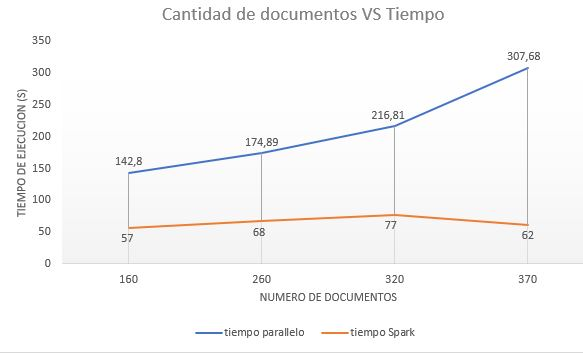
\includegraphics[width=\linewidth]{graficaParalellovsSpark}
	\caption{Gráfico HPC Vs. Spark}
	\label{fig:graficoParaleloVsSpark}
\end{figure*}

\section{Implementación}
La implementación de esta practica fue realizada en python ya que es un lenguaje de programación muy sencillo de utilizar pero principalmente por que es un lenguaje sobre el cual se tiene mas experiencia.
Para la implementacíon del codigo se utilizo PySpark y ademas se utilizaron algunas bibliotecas como sys, math, numpy, pyspark.sql, pyspark.mllib y pyspark.mllib que nos permitieron realizar operaciones como lectura de ficheros, manejo de argumentos, estructuras de datos para facilitar el ordenamiento, almacenamiento y procesamiento de los datos, tambien se empleo numpy como un soporte para las estructuras de datos necesarias para la matriz que contenia todas las distancias entre documentos.


A continuación compartimos nuestra implementación alojada en Github, en la cual basamos el análisis presentado en este estudio; al interior de este link podra encontrar un Readme.md con todas las instrucciones necesarias por poder correr satisfactoriamente los diferentes algoritmos: \href{https://github.com/jonyzp/Spark-Document-Clustering}{Repositorio de Github}

\section{Análisis de resultados (Spark vs. HPC)}

A continuación presentamos el gráfico resultante del proceso de medición, el cual evidencia las aceleraciones entre datasets e implementaciones y en distintas ejecuciones.

\begin{table}[hbt]
	\caption{Tabla de Comparaciones de tiempo}
	\centering
	\begin{tabular}{llr}
%		\toprule
%		\multicolumn{1}{c}{Parámetro de comparación} \\
		\cmidrule(r){1-3}
		SetSize (MB) & T. Spark (seg) & T. Paralelo (seg)\\
		\midrule
		
		119,92 & 107 & 307,68 \\
		
		94,88 & 71 & 216,81 \\
		
		75,02 & 60 & 174,89 \\
		
		68,66 & 55 & 142,80 \\
		
		\bottomrule
	\end{tabular}
	\label{tab:label}
\end{table}


Se puede evidenciar la diferencia entre ejecutar el algoritmo que es diseñado y ejecutado en clusters de Computación de Alto Rendimiento a ejecutar el software implementado sobre Spark, aunque el algoritmo paralelo tiene un mayor orden de complejidad, logra reducir el tiempo que tardaria en dar la solución un algoritmo serial, ya que el procesamiento se realiza de una manera distribuída, pero aun asi no logra superar los tiempos que nos arroja ejecutarlo sobre un cluster donde se encuentra configurada correctamente la tecnologia Spark.


%------------------------------------------------
\phantomsection
\section*{Conclusiones} % The \section*{} command stops section numbering

\begin{itemize}
	\item Creemos que lo mas importante que se debe de resaltar aquí, es la gran diferencia que tienen ambas implementaciones en cuanto a la facilidad de desarrollo.
	\item  Al ser Spark una tecnologia enfocada para trabajar de forma facil con HDFS, permite al usuario analizar una gran cantidad de archivos que se encuentran de forma distribuida sin influir de forma muy directa la programación de la implementación.
	\item La Forma en la que Spark procesa los datos hace que inclusive la ejecución sobre 4 nodos de procesamiento demore menos que la ejecución sobre 50 nodos de procesamaiento que se hizo en HPC.
\end{itemize}
% So long and thanks for all the fish \cite{Figueredo:2009dg}.

%----------------------------------------------------------------------------------------
%	REFERENCE LIST
%----------------------------------------------------------------------------------------


\begin{thebibliography}{9}

\bibitem{K-means}
Alsabti, K., Ranka, S. and Singh, V. (2017). An Efficient K-Means Clustering Algorithm. [online] pp.1-2. \href{https://www.cs.utexas.edu/~kuipers/readings/Alsabti-hpdm-98.pdf}{Available clicking here} [Accessed 22 Oct. 2017].
\bibitem{K-means Algorithm}
Home.deib.polimi.it. (2017). Clustering - K-means. [online] \href{http://home.deib.polimi.it/matteucc/Clustering/tutorial_html/kmeans.html}{Available clicking here} [Accessed 22 Oct. 2017].
 
\bibitem{document clustering}
En.wikipedia.org. (2017). Document clustering. [online] \href{https://en.wikipedia.org/wiki/Document_clustering}{Available clicking here} [Accessed 22 Oct. 2017].

\bibitem{Doc_clust_techniques} 
Glaros.dtc.umn.edu. (2017). A Comparison of Document Clustering Techniques | Karypis Lab. [online] \href{http://glaros.dtc.umn.edu/gkhome/node/157}{Available clicking here} [Accessed 22 Oct. 2017].

\bibitem{hpc} 
insideHPC. (2017). What is high performance computing? - insideHPC. [online] \href{https://insidehpc.com/hpc-basic-training/what-is-hpc/}{Available clicking here}  [Accessed 22 Oct. 2017].

\bibitem{hpc_def} 
SearchDataCenter. (2017). What is high-performance computing (HPC)? - Definition from WhatIs.com. [online] 
\href{http://searchdatacenter.techtarget.com/definition/high-performance-computing-HPC}{Available clicking here}   [Accessed 22 Oct. 2017].



\bibitem{parallel_comp_lawrence_nat_lab} 
Computing.llnl.gov. (2017). Introduction to Parallel Computing. [online] \href{https://computing.llnl.gov/tutorials/parallel_comp/}{Available clicking here}  [Accessed 22 Oct. 2017].


\bibitem{Parallel Computing}
Types of Parallelism. [online] \href{http://www.inf.ed.ac.uk/teaching/courses/pa/Notes/lecture02-types.pdf}{Available clicking here} [Accessed 22 Oct. 2017].

\end{thebibliography}


%----------------------------------------------------------------------------------------


% no BORRAR:
%\begin{verbatim}
%CODE HERE
%\end{verbatim}


\end{document}
